\documentclass{standalone}
\usepackage{tikz}
\usetikzlibrary{positioning, arrows.meta, shapes.geometric, fit, calc}
\usepackage{pgfplots}
\usepackage{duckuments}
\pgfplotsset{compat=1.18}

\begin{document}
\begin{tikzpicture}[
        node distance=1.5cm,
        box/.style={rectangle, draw, minimum height=1.8cm, minimum width=1.4cm,
                align=center},
        activation/.style={rectangle, draw, rounded corners, minimum width=1.4cm,
                minimum height=1.8cm, fill=orange!20, align=center},
        arrow/.style={-Stealth, thick},
        data/.style={rectangle, draw, minimum height=1.8cm, minimum width=1.4cm,
                rounded corners, fill=blue!10, align=center}
    ]

    % First row - Classification pipeline
    % Input image visualization
    \node[draw, minimum width=0.8cm, minimum height=0.8cm] (input) {
        % \begin{tikzpicture}
        %     \node[inner sep=0] {
        %         \begin{tikzpicture}[scale=0.4]
        %             % Simple digit "7" image
        %             \fill[black] (0,0) rectangle (2,0.5);
        %             \fill[black] (1.5,0) rectangle (2,2);
        %             \fill[black] (1,1.5) rectangle (2,2);
        %             \fill[black] (1.5,2) rectangle (1.5,2);
        %             \fill[black] (1,1.5) rectangle (2,2);
        %             \fill[black] (0.5,1) rectangle (1.5,1.5);

        %             % Grid lines to show pixels
        %             \draw[gray, thin] (0,0) grid (2,2);
        %         \end{tikzpicture}
        %     };
        %     \node[above] at (0,0.4) {Sample Image};
        % \end{tikzpicture}
        \includegraphics[width=0.3\linewidth]{example-image-duck}
    };

    \node[box, right=of input, fill=yellow!10] (linear) {Linear\\FC Layer};
    \node[activation, right=of linear] (relu) {ReLU\\Activation};
    \node[box, right=of relu, fill=green!10] (softmax) {Softmax};

    % Output probabilities - now numerically ordered with ellipses
    \node[right=of softmax] (output) {
        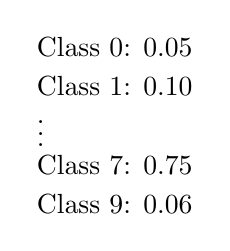
\begin{tikzpicture}
            % Numerically ordered list of probabilities with ellipses
            \node[anchor=west] at (0,1.0) {Class 0: 0.05};
            \node[anchor=west] at (0,0.5) {Class 1: 0.10};
            \node[anchor=west] at (0,0.0) {$\vdots$};
            \node[anchor=west] at (0,-0.5) {Class 7: 0.75};
            \node[anchor=west] at (0,-1.0) {Class 9: 0.06};
        \end{tikzpicture}
    };

    % Connections in first row
    \draw[arrow] (input) -- (linear);
    \draw[arrow] (linear) -- (relu);
    \draw[arrow] (relu) -- (softmax);
    \draw[arrow] (softmax) -- (output);

    % Second row - Simple PCA visualization with just three clusters
    % \node[below=2.5cm of relu] (pca) {
    %     \begin{tikzpicture}
    %         \begin{axis}[
    %             width=7cm, height=6cm,
    %             title={PCA of Activation Values},
    %             xlabel={Principal Component 1},
    %             ylabel={Principal Component 2},
    %             xmin=-3, xmax=3,
    %             ymin=-3, ymax=3,
    %             grid=both,
    %             legend style={at={(0.97,0.03)}, anchor=south east}
    %         ]

    %         % Fixed: Adding explicit draw=black to make borders visible
    %         % Cluster for "0"
    %         \addplot[only marks, mark=o, mark size=3pt, draw=black, fill=blue, opacity=0.7] coordinates {
    %             (-2.3, -1.8) (-2.1, -2.0) (-2.5, -1.9) (-2.2, -1.7) (-2.4, -2.1)
    %             (-2.0, -1.6) (-2.6, -2.2) (-2.3, -1.5) (-2.7, -1.7) (-1.9, -1.9)
    %         };

    %         % Cluster for "1"
    %         \addplot[only marks, mark=square, mark size=3pt, draw=black, fill=red, opacity=0.7] coordinates {
    %             (2.1, 1.7) (2.3, 1.9) (2.0, 1.8) (2.4, 1.6) (2.2, 2.0)
    %             (1.9, 1.5) (2.5, 1.8) (2.1, 2.1) (2.3, 1.6) (2.6, 1.7)
    %         };

    %         % Cluster for "7"
    %         \addplot[only marks, mark=diamond, mark size=3pt, draw=black, fill=green!60!black, opacity=0.7] coordinates {
    %             (0.2, 2.5) (0.4, 2.7) (0.1, 2.6) (0.5, 2.8) (0.3, 2.4)
    %             (0.0, 2.3) (0.6, 2.5) (0.2, 2.9) (-0.1, 2.7) (0.4, 2.2)
    %         };

    %         % Labels
    %         \node[blue] at (-2.3,-1.4) {} ;
    %         \node[red] at (2.2,1.3) {};
    %         \node[green!60!black] at (0.2,2.1) {};

    %         \end{axis}
    %     \end{tikzpicture}
    % };

    \node[below=2.5cm of relu] (pca) {
        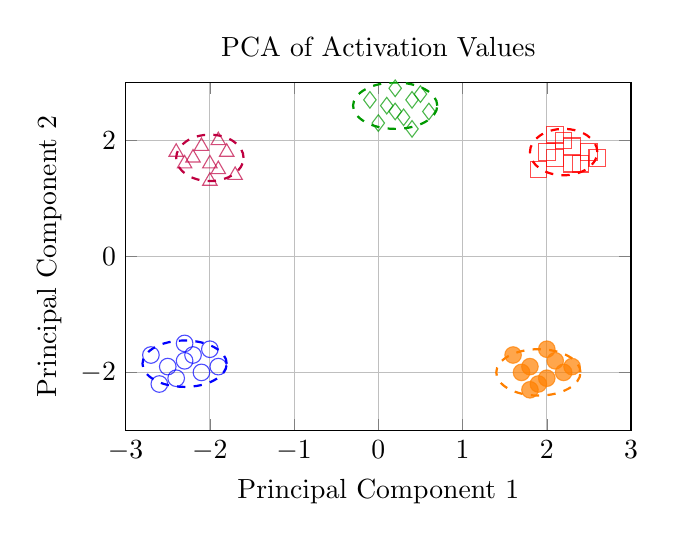
\begin{tikzpicture}
            \begin{axis}[
                    width=8cm, height=6cm,
                    title={PCA of Activation Values},
                    xlabel={Principal Component 1},
                    ylabel={Principal Component 2},
                    xmin=-3, xmax=3,
                    ymin=-3, ymax=3,
                    grid=both,
                    legend style={at={(0.97,0.03)}, anchor=south east},
                    scatter/use mapped color={draw=black},
                ]

                % Improved visualization with clusters and labels
                % Digit 0
                \addplot[only marks, mark=o, mark size=3pt, color=blue, opacity=0.7]
                coordinates {
                        (-2.3, -1.8) (-2.1, -2.0) (-2.5, -1.9) (-2.2, -1.7) (-2.4, -2.1)
                        (-2.0, -1.6) (-2.6, -2.2) (-2.3, -1.5) (-2.7, -1.7) (-1.9, -1.9)
                    };

                % Digit 1
                \addplot[only marks, mark=square, mark size=3pt, color=red,
                    opacity=0.7] coordinates {
                        (2.1, 1.7) (2.3, 1.9) (2.0, 1.8) (2.4, 1.6) (2.2, 2.0)
                        (1.9, 1.5) (2.5, 1.8) (2.1, 2.1) (2.3, 1.6) (2.6, 1.7)
                    };

                % Digit 7
                \addplot[only marks, mark=diamond, mark size=3pt, color=green!60!black,
                    opacity=0.7] coordinates {
                        (0.2, 2.5) (0.4, 2.7) (0.1, 2.6) (0.5, 2.8) (0.3, 2.4)
                        (0.0, 2.3) (0.6, 2.5) (0.2, 2.9) (-0.1, 2.7) (0.4, 2.2)
                    };

                % Digit 4
                \addplot[only marks, mark=triangle, mark size=3pt, color=purple,
                    opacity=0.7] coordinates {
                        (-2.0, 1.6) (-1.8, 1.8) (-2.2, 1.7) (-1.9, 1.5) (-2.1, 1.9)
                        (-1.7, 1.4) (-2.3, 1.6) (-1.9, 2.0) (-2.0, 1.3) (-2.4, 1.8)
                    };

                % Digit 9
                \addplot[only marks, mark=*, mark size=3pt, color=orange, opacity=0.7]
                coordinates {
                        (1.8, -1.9) (2.0, -2.1) (1.7, -2.0) (2.1, -1.8) (1.9, -2.2)
                        (1.6, -1.7) (2.2, -2.0) (1.8, -2.3) (2.0, -1.6) (2.3, -1.9)
                    };

                % Add ellipses around clusters
                \draw[blue, thick, dashed] (-2.3,-1.85) ellipse (0.5 and 0.4);
                \draw[red, thick, dashed] (2.2,1.8) ellipse (0.4 and 0.4);
                \draw[green!60!black, thick, dashed] (0.2,2.6) ellipse (0.5 and 0.4);
                \draw[purple, thick, dashed] (-2.0,1.7) ellipse (0.4 and 0.4);
                \draw[orange, thick, dashed] (1.9,-2.0) ellipse (0.5 and 0.4);

                % Labels
                \node[blue] at (-2.3,-1.4) {};
                \node[red] at (2.2,1.3) {};
                \node[green!60!black] at (0.2,2.1) {};
                \node[purple] at (-2.0,1.2) {};
                \node[orange] at (1.9,-1.5) {};

            \end{axis}
        \end{tikzpicture}
    };

    % Arrow from ReLU to PCA
    \draw[arrow] (relu) -- (pca);
    % \node[right] at ($(relu)!0.5!(pca) + (0.5,0)$) {Visualize Activations};

\end{tikzpicture}
\end{document}